\documentclass{article}
\usepackage{listings}
\usepackage{listings}
\usepackage{color}
\usepackage{graphicx}
\usepackage{caption}
\graphicspath{ {./} }
\usepackage[top=1in, bottom=1.25in, left=1.25in, right=1.25in]{geometry}
\definecolor{mygreen}{rgb}{0,0.6,0}
\definecolor{mygray}{rgb}{0.5,0.5,0.5}
\definecolor{mymauve}{rgb}{0.58,0,0.82}
\lstset{ %
	backgroundcolor=\color{white},   % choose the background color; you must add \usepackage{color} or \usepackage{xcolor}; should come as last argument
	basicstyle=\footnotesize,        % the size of the fonts that are used for the code
	breakatwhitespace=false,         % sets if automatic breaks should only happen at whitespace
	breaklines=true,                 % sets automatic line breaking
	captionpos=b,                    % sets the caption-position to bottom
	commentstyle=\color{mygreen},    % comment style
	deletekeywords={...},            % if you want to delete keywords from the given language
	escapeinside={\%*}{*)},          % if you want to add LaTeX within your code
	extendedchars=true,              % lets you use non-ASCII characters; for 8-bits encodings only, does not work with UTF-8
	frame=single,	                   % adds a frame around the code
	keepspaces=true,                 % keeps spaces in text, useful for keeping indentation of code (possibly needs columns=flexible)
	keywordstyle=\color{blue},       % keyword style
	language=Octave,                 % the language of the code
	morekeywords={*,...},            % if you want to add more keywords to the set
	numbers=left,                    % where to put the line-numbers; possible values are (none, left, right)
	numbersep=5pt,                   % how far the line-numbers are from the code
	numberstyle=\tiny\color{mygray}, % the style that is used for the line-numbers
	rulecolor=\color{black},         % if not set, the frame-color may be changed on line-breaks within not-black text (e.g. comments (green here))
	showspaces=false,                % show spaces everywhere adding particular underscores; it overrides 'showstringspaces'
	showstringspaces=false,          % underline spaces within strings only
	showtabs=false,                  % show tabs within strings adding particular underscores
	stepnumber=2,                    % the step between two line-numbers. If it's 1, each line will be numbered
	stringstyle=\color{mymauve},     % string literal style
	tabsize=2,	                   % sets default tabsize to 2 spaces
	title=\lstname                   % show the filename of files included with \lstinputlisting; also try caption instead of title
}
\author{Polykarpos Thomadakis}
\title{Assignment 2 \\
	\large CS834 Introduction to Information Retrieval\\Fall 2017}
\begin{document}
	\maketitle
	\section*{Question 4.1}
	Plot rank-frequency curves (using a log-log graph) for words and bigrams in
	the Wikipedia collection available through the book website ( http://www.search-
	engines-book.com ). Plot a curve for the combination of the two. What are the best
	values for the parameter c for each curve?
	\subsection*{Answer}
	To answer this question, I wrote a Python script that parses each documents in the Wikipedia collection and extracts all of its tokens. Then, count the frequency of each token, create bigrams from those tokens and count the frequency of the bigrams.\\ Finally, for both tokens and bigrams rank them by their frequency and compute their probability and the 'c' value.
	The output is written on a csv file for easier visualization into tables. For the purposes of this assignment I used the Wiki small collection of the book's website. \\The script can be found in listing \ref{lst:word_freq}.
	
	\lstinputlisting[language=Python,caption={Script to extract toke and bigram information},label={lst:word_freq}]{word_freq.py}
	
	The top 10 tokens in terms of frequency are shown in Table \ref{tb:token_freq} . In file results.csv you can find the complete results for the tokens' frequency ranking in this collection. Table \ref{tb:bigram_freq} shows the same information for the case of the bigrams as can be also found in results\_bigrams.csv. To generate the requested graphs I used gnuplot on the results.csv, results\_bigrams.csv files. The log-log rank-frequency plots for the tokens, bigrams and their comparison are presented in Figures \ref{fig:tokens_log}, \ref{fig:bigrams_log} and \ref{fig:comparison_log}, respectively.
	
	\begin{table}[h]
		\centering
		\caption{Top ten ranked tokens in Wiki small collection}
		\label{tb:token_freq}
		\resizebox{\columnwidth}{!}{
		\begin{tabular}{lllll}
			Rank & Frequency & Word      & Probability           & c                    \\
			1    & 169695    & the       & 0.038954823010881046  & 0.038954823010881046 \\
			2    & 111772    & of        & 0.025658142417703502  & 0.051316284835407004 \\
			3    & 77940     & and       & 0.01789174050778201   & 0.05367522152334603  \\
			4    & 62273     & a         & 0.014295257334373996  & 0.057181029337495984 \\
			5    & 60351     & Wikipedia & 0.01385404710527524   & 0.06927023552637619  \\
			6    & 59125     & in        & 0.013572609154767917  & 0.08143565492860749  \\
			7    & 54327     & to        & 0.012471190487121803  & 0.08729833340985262  \\
			8    & 41122     & is        & 0.009439878793443827  & 0.07551903034755061  \\
			9    & 33865     & by        & 0.0077739773196822915 & 0.06996579587714062  \\
			10   & 31434     & The       & 0.007215922133969974  & 0.07215922133969974 
		\end{tabular}
		}
	\end{table}
		\begin{table}[]
			\centering
			\caption{Top ten ranked bigrams in Wiki small collection}
			\label{tb:bigram_freq}
			\resizebox{\columnwidth}{!}{
			\begin{tabular}{lllll}
				Rank & Frequency & Word                     & Probability           & c                    \\
				1    & 37574     & ('of', 'the')            & 0.008625407465221982  & 0.008625407465221982 \\
				2    & 15151     & ('in', 'the')            & 0.003478031311693678  & 0.010434093935081035 \\
				3    & 14010     & ('is', 'a')              & 0.0032161057802672054 & 0.012864423121068821 \\
				4    & 12147     & ('the', 'free')          & 0.0027884394655892752 & 0.013942197327946377 \\
				5    & 12088     & ('free', 'encyclopedia') & 0.0027748955511684497 & 0.016649373307010697 \\
				6    & 12088     & ('Wikipedia', 'the')     & 0.0027748955511684497 & 0.019424268858179147 \\
				7    & 12086     & ('About', 'Wikipedia')   & 0.0027744364354253706 & 0.027744364354253707 \\
				8    & 10932     & ('Wikipedia', 'user')    & 0.0025095266516688857 & 0.03011431982002663  \\
				9    & 10932     & ('by', 'Wikipedia')      & 0.0025095266516688857 & 0.032623846471695514 \\
				10   & 9622      & ('user', 's')            & 0.002208805839952252  & 0.030923281759331532
			\end{tabular}
			}
		\end{table}
		\begin{figure}[]
			\begin{minipage}{.45\textwidth}
				\centering
				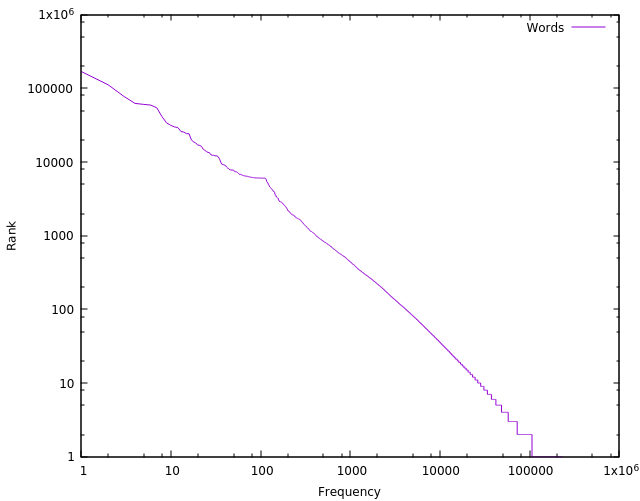
\includegraphics[width=\linewidth]{words_graph.png}
				
				\captionof{figure}{The rank-frequency curve for the words in the Wiki small collection}
				\label{fig:tokens_log}
			\end{minipage}
			\begin{minipage}{.45\textwidth}
				\centering
				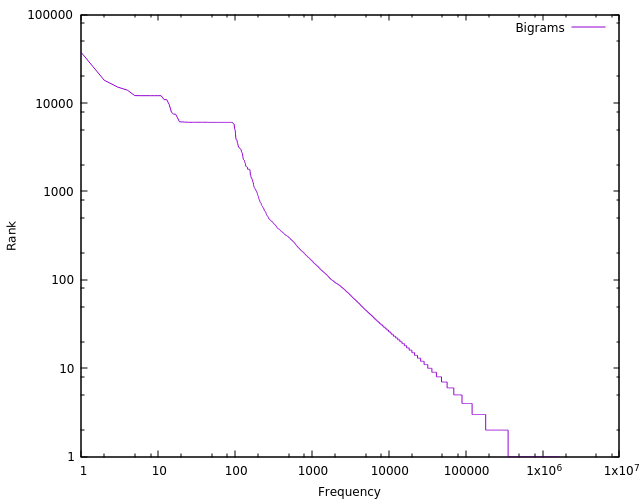
\includegraphics[width=\linewidth]{bigrams_graph.png}
				\captionof{figure}{The rank-frequency curve for the bigrams in the Wiki small collection}
				\label{fig:bigrams_log}
			\end{minipage}
			\begin{minipage}{.45\textwidth}
				\centering
				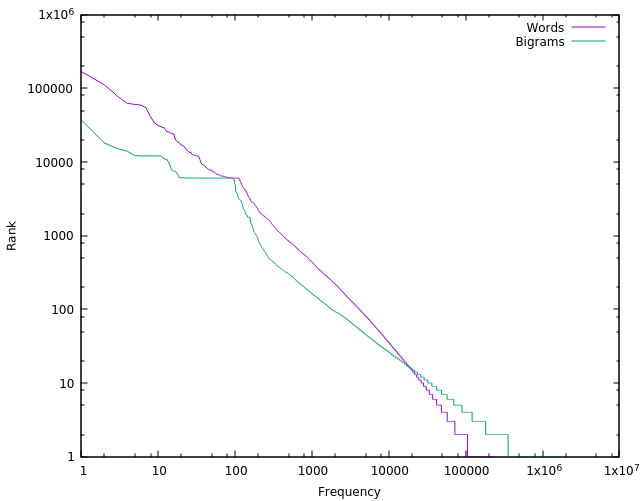
\includegraphics[width=\linewidth]{word_bigrams_graph.png}
				\captionof{figure}{The rank-frequency curve for the bigrams and words in the Wiki small collection}
				\label{fig:comparison_log}
			\end{minipage}
		\end{figure}
		\section*{Question 4.2}
		Plot vocabulary growth for the Wikipedia collection and estimate the parameters for Heaps’ law. Should the order in which the documents are processed make any difference?
		\subsection*{Answer}
		For this assignment we should count the number of words per document and the number of unique words. This way we have a analogy between the total number of words and the number of unigue words in different points steps of parsing the collection of documents. I used the Wiki small collection again. The script used is shown in listing \ref{lst:voc_growth}. It can take as option argument the -r option that will make it parse the documents in reverse order for the purposes of this assignment. 
		The parameters that need to be defined are k and $\beta$ from Heap's law:$$v=kn^{\beta}$$
		In order to estimate those values, I used non-linear least square fitting from python. The script used for this purpose is presented in listing \ref{lst:fitting}. The curves produced by using the values found from this fitting and the curves generated by the experiments are shown in figure \ref{fig:heaps_law} and figure \ref{fig:heaps_law_rev}. Using this methodology I get the results shown in table \ref{tb:order_rev}, which point out that the order in which the files are visited can impact the vocabulary growth curve.
		\lstinputlisting[language=Python,caption={Script to extract the vocabulary growth information},label={lst:voc_growth}]{voc_growth.py}
		\lstinputlisting[language=Python,caption={Script that calculates the parameters of Heap's law using non-linear least square fitting},label={lst:fitting}]{fit.py}
		\begin{table}[h]
			\centering
			\caption{Heap's law parameters}
			\label{tb:order_rev}
			\begin{tabular}{|l|l|l|}
				\hline
				& In order & Reverse \\ \hline
				k       & 25.1230  & 6.807   \\ \hline
				$\beta$ & 0.597    & 0.680  \\ \hline
			\end{tabular}
		\end{table}
		\begin{figure}[]
			\begin{minipage}{.45\textwidth}
				\centering
				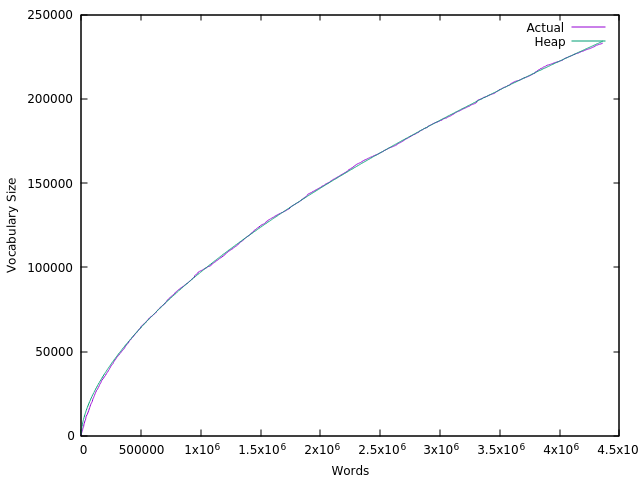
\includegraphics[width=\linewidth]{heap_actual.png}
				\captionof{figure}{The vocabulary growth for the Wiki small collection}
				\label{fig:heaps_law}
			\end{minipage}
			\begin{minipage}{.45\textwidth}
				\centering
				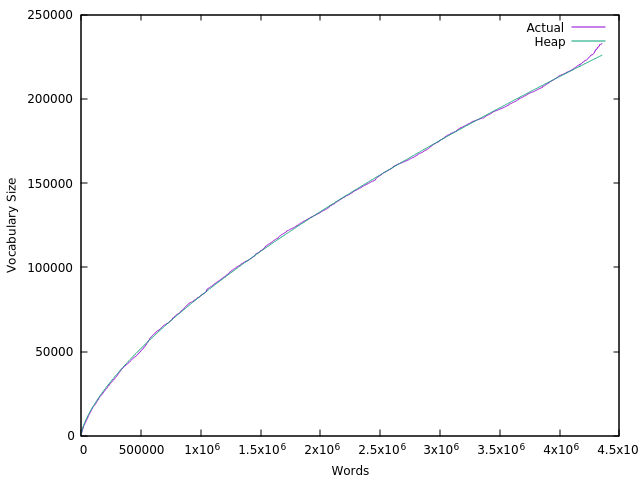
\includegraphics[width=\linewidth]{heap_actual_reverse.png}
				\captionof{figure}{The vocabulary growth for the Wiki small collection parsed in reverse order}
				\label{fig:heaps_law_rev}
			\end{minipage}
		\end{figure}
		
		
		
		\section*{Question 4.6}
		Process five Wikipedia documents using the Porter stemmer and the Krovetz stemmer. Compare the number of stems produced and find 10 examples of differences in the stemming that could have an impact on ranking.
		\subsection*{Answer}
		The  five documents I chose for this assignment are shown below in table \ref{tb:html_files} with the number of stems per algorithm. 	I use existing Python's libraries to retrieve the results of both stemming algorithms. Krovetz's algorithm is more sophisticated and this can be realized by the 10 differences presented in table \ref{tb:term_diffs}. As one can notice, Porter stemming produces many stems that have no meaning in English, thus, impacting the overalll ranking of the document. The script used to collect this information is given in listing \ref{lst:port_krov}. This scripts produces 2 files per original document, containing the Porter and Krovatz stemming respectively. The output can be found in my github repository in filenames ending in .krovetz or .porter.
		\begin{table}[]
			\centering
			\caption{Comparison between the two stemming algorithms for the five html files chosen}
			\label{tb:html_files}
			\begin{tabular}{|l|l|l|l|}
				\hline
				No & File                          & Porter stems \# & Krovetz stems \# \\ \hline
				1  & Agia\_Dynati\_f24a.html       & 230             & 227              \\ \hline
				2  & Agnes\_of\_Glasgow\_3312.html & 346             & 342              \\ \hline
				3  & Agoranomos.html               & 454             & 450              \\ \hline
				4  & Astolfo.html                  & 628             & 632              \\ \hline
				5  & Parand.html                   & 738             & 746              \\ \hline
			\end{tabular}
		\end{table}
	    \begin{table}[b]
	    	\centering
	    	\caption{Ten differences in the stems produced by the 2 algorithms}
	    	\label{tb:term_diffs}
	    	\begin{tabular}{|l|l|l|}
	    		\hline
	    		Original & Porter  & Krovetz  \\ \hline
	    		produces & produc  & produce  \\ 
	    		believe  & believ  & believe  \\ 
	    		greece   & greec   & greece   \\ 
	    		because  & becaus  & because  \\ 
	    		his      & hi      & his      \\ 
	    		zeus     & zeu     & zeus     \\ 
	    		during   & dure    & during   \\ 
	    		infamous & infam   & infamous \\ 
	    		massacre & massacr & massacre \\ 
	    		division & divis   & division \\ \hline
	    	\end{tabular}
	    \end{table}
		\lstinputlisting[language=Python,caption={Script to extract stems from the 5 documents using the two given algorithms},label={lst:port_krov}]{porter_krovetz.py}
		\section*{Question 4.8}
		Find the 10 Wikipedia documents with the most inlinks. Show the collection of anchor text for those pages.
		\subsection*{Answer}
		The methodology for this assignment is to parse all files in the Wiki small collection, maintaining a dictionary of documents to number of inlinks and another of inlinks to anchor texts. Once all files have been parsed, the first dictionary is sorted by the number of inlinks and then the second dictionary is printed based on the order that the first dictionary has given to its keys. Only the links that point to file in the collection are considered for this assignment. The results of the algorithm can are presented in table \ref{tb:inlink_cnt}. The Python script for this assignment is presented in listing \ref{lst:inlinks}
		\begin{table}[]
			\centering
			\caption{Top ten documents with the most inlinks with their anchors}
			\label{tb:inlink_cnt}
			\resizebox{\columnwidth}{!}{
			\begin{tabular}{|l|l|l|l|}
				\hline
				\textbf{No} & \textbf{Inlinks \#} & \textbf{Document}                                               & \textbf{Anchor texts}                                        \\ \hline
				1           & 123                 & en/articles/b/r/a/Brazil.html                                   & Brazil,BRA,Brazilian                                         \\ \hline
				2           & 44                  & en/articles/a/u/g/August\_26.html                               & 08-26,26,August 26,26 August                                 \\ \hline
				3           & 17                  & en/articles/m/a/n/Manga.html                                    & manga,Manga                                                  \\ \hline
				4           & 14                  & en/articles/m/a/g/Magazine.html                                 & magazine,magazines,Magazine                                  \\ \hline
				5           & 12                  & en/articles/m/o/l/Mollusca.html                                 & Mollusca                                                     \\ \hline
				6           & 11                  & en/articles/v/i/c/Victoria\_of\_the\_United\_Kingdom\_5e8e.html & Victoria,Queen,Victoria of the United Kingdom,Queen Victoria \\ \hline
				7           & 8                   & en/articles/s/c/r/Screenwriter.html                             & Writer(s),screenwriter,Screenwriter                          \\ \hline
				8           & 7                   & en/articles/t/u/s/Tuscany.html                                  & Tuscany                                                      \\ \hline
				9           & 6                   & en/articles/k/i/d/Kidney.html                                   & kidneys,Renal,kidney                                         \\ \hline
				10          & 6                   & en/articles/t/o/t/Tottenham\_Hotspur\_F.C.\_6bd2.html           & Tottenham Hotspur,Tottenham                                  \\ \hline
			\end{tabular}}
		\end{table}
		\lstinputlisting[language=Python,caption={Script to extract the top 10 documents with most inlinks and their anchor texts},label={lst:inlinks}]{inlinks.py}
		\section*{Question 5.8}
		Write a program that can build a simple inverted index of a set of text docu-
		ments. Each inverted list will contain the file names of the documents that contain
		that word.
		Suppose the file A contains the text “the quick brown fox”, and file B contains
		“the slow blue fox”. The output of your program would be:
		\begin{verbatim}
		% ./your-program A B
		blue B
		brown A
		fox A B
		quick A
		slow B
		the A B
		\end{verbatim}
		\subsection*{Answer}
		In order to create the inverted index, I parse all the documents given, maintaining a dictionary of tokens to sets of files. For each token I keep all the documents that contain this term. The script used takes as command argument a list of documents to parse, or a filepath to search for all .html files below it and creates a file containing the inverted index. A part of the file produced is shown in table \ref{tb:inv_index}. I used the files Enayetpur.html,Gabrias.html for this assignment. The script that generates the inverted index is presented in listing \ref{lst:inv_index}
		\lstinputlisting[language=Python,caption={Script to create an inverted index},label={lst:inv_index}]{inv_index.py}
		\begin{table}[h]
			\centering
			\caption{The 30 first rows of the inverted index produced}
			\label{tb:inv_index}
			\begin{tabular}{|l|l|}
				\hline
				\multicolumn{1}{|l|}{Token} & \multicolumn{1}{l|}{Documents} \\ \hline
				Based                       & Enayetpur.html,Gabrias.html    \\
				help                        & Enayetpur.html,Gabrias.html    \\
				just                        & Enayetpur.html                 \\
				text                        & Enayetpur.html,Gabrias.html    \\
				Coordinates                 & Gabrias.html                   \\
				produced                    & Enayetpur.html                 \\
				sources                     & Enayetpur.html                 \\
				geography                   & Gabrias.html                   \\
				adding                      & Enayetpur.html                 \\
				Recently                    & Enayetpur.html                 \\
				also                        & Enayetpur.html                 \\
				Navigation                  & Enayetpur.html,Gabrias.html    \\
				7EMonobook                  & Enayetpur.html,Gabrias.html    \\
				YUNUS                       & Enayetpur.html                 \\
				Here                        & Enayetpur.html                 \\
				thana                       & Enayetpur.html                 \\
				to                          & Enayetpur.html,Gabrias.html    \\
				window                      & Enayetpur.html,Gabrias.html    \\
				Alaibot                     & Gabrias.html                   \\
				Nederlands                  & Gabrias.html                   \\
				rich                        & Enayetpur.html                 \\
				under                       & Enayetpur.html,Gabrias.html    \\
				SieBot                      & Gabrias.html                   \\
				main                        & Enayetpur.html,Gabrias.html    \\
				geographical                & Gabrias.html                   \\
				lacking                     & Enayetpur.html                 \\
				Khukni                      & Enayetpur.html                 \\
				LordAnubisBOT               & Gabrias.html                   \\
				material                    & Enayetpur.html                 \\
				deductible                  & Enayetpur.html,Gabrias.html    \\ \hline
			\end{tabular}
		\end{table}
		
		
\end{document}